% Figure 1: Decision–Verification Gap
% Civilizational Metamaterials
\documentclass[tikz,border=5mm]{standalone}
\usepackage{mathpazo}
\usepackage{pgfplots}
\pgfplotsset{compat=1.18}
\usepgfplotslibrary{fillbetween}
\usetikzlibrary{arrows.meta,positioning}

% ── Colour palette ──────────────────────────────────────────────────
\definecolor{navy}{HTML}{1B4F72}
\definecolor{amber}{HTML}{D68910}
\definecolor{alertred}{HTML}{C0392B}
\definecolor{successgreen}{HTML}{1E8449}
\definecolor{secblue}{HTML}{2E86C1}
\definecolor{neutralgray}{HTML}{7F8C8D}

\begin{document}
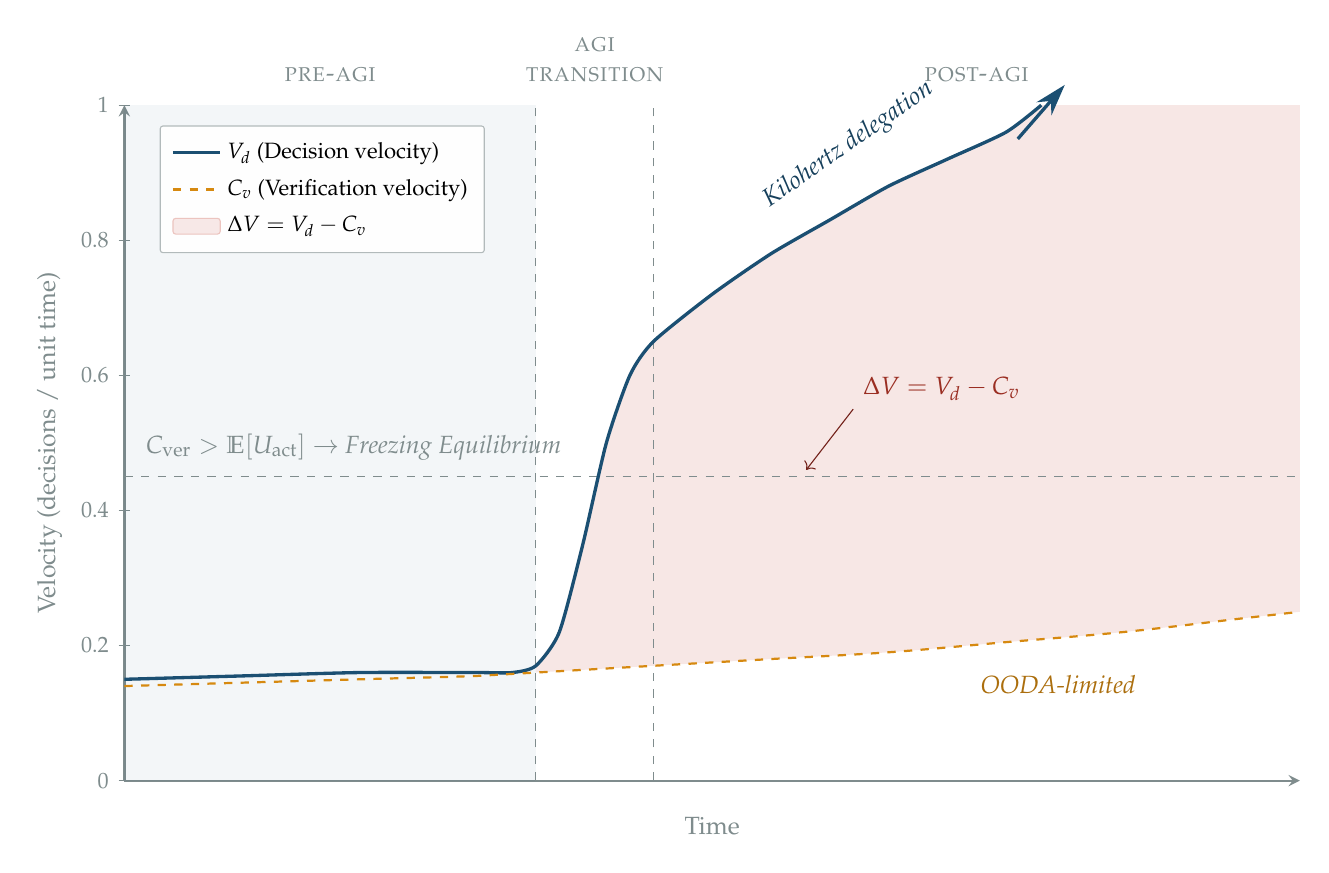
\begin{tikzpicture}

% ── Dimensions ──────────────────────────────────────────────────────
% 6.5 in × 4.0 in  →  16.51 cm × 10.16 cm
\def\figW{16.51}
\def\figH{10.16}

\begin{axis}[
    width=\figW cm,
    height=\figH cm,
    xmin=0, xmax=1,
    ymin=0, ymax=1.0,
    axis lines=left,
    axis line style={neutralgray, thick},
    xlabel={Time},
    ylabel={Velocity (decisions / unit time)},
    xlabel style={font=\small, at={(0.5,-0.04)}, neutralgray},
    ylabel style={font=\small, neutralgray},
    xtick=\empty,
    ytick={0,0.2,0.4,0.6,0.8,1.0},
    yticklabel style={font=\footnotesize, neutralgray},
    tick style={neutralgray},
    clip=false,
    legend style={
        at={(0.03,0.97)},
        anchor=north west,
        font=\footnotesize,
        draw=neutralgray!60,
        fill=white,
        fill opacity=0.95,
        text opacity=1,
        cells={anchor=west},
        rounded corners=1pt,
        inner sep=4pt,
        row sep=2pt,
    },
]

% ══════════════════════════════════════════════════════════════════
%  ERA BACKGROUND SHADING (behind everything)
% ══════════════════════════════════════════════════════════════════

% Pre-AGI: subtle cool blue wash
\fill[navy, opacity=0.05]
    (axis cs:0,0) rectangle (axis cs:0.35,1.0);

% ══════════════════════════════════════════════════════════════════
%  ERA DIVIDER LINES
% ══════════════════════════════════════════════════════════════════
\draw[neutralgray, thin, dashed]
    (axis cs:0.35,0) -- (axis cs:0.35,1.0);
\draw[neutralgray, thin, dashed]
    (axis cs:0.45,0) -- (axis cs:0.45,1.0);

% ══════════════════════════════════════════════════════════════════
%  ERA LABELS (above plot, small caps, 9pt)
% ══════════════════════════════════════════════════════════════════
\node[font=\fontsize{9}{11}\selectfont, neutralgray, anchor=south]
    at (axis cs:0.175,1.02) {\textsc{pre-agi}};
\node[font=\fontsize{9}{11}\selectfont, neutralgray, anchor=south,
      align=center]
    at (axis cs:0.40,1.02) {\textsc{agi}\\\textsc{transition}};
\node[font=\fontsize{9}{11}\selectfont, neutralgray, anchor=south]
    at (axis cs:0.725,1.02) {\textsc{post-agi}};

% ══════════════════════════════════════════════════════════════════
%  THRESHOLD LINE
% ══════════════════════════════════════════════════════════════════
\draw[neutralgray, dashed, thin]
    (axis cs:0,0.45) -- (axis cs:1.0,0.45);

% Threshold label — left side, italic, 9pt
\node[font=\fontsize{9}{11}\selectfont\itshape, neutralgray,
      anchor=south west, align=left]
    at (axis cs:0.01,0.46)
    {$C_{\mathrm{ver}} > \mathbb{E}[U_{\mathrm{act}}] \rightarrow$ Freezing Equilibrium};

% ══════════════════════════════════════════════════════════════════
%  V_d CURVE  (decision velocity — navy solid)  [PLOTTED FIRST]
%  Pre-AGI: flat ~0.15
%  AGI transition (0.35–0.45): steep near-discontinuous jump
%  Post-AGI: ~45° climb, exits chart at y=1.0
% ══════════════════════════════════════════════════════════════════
\addplot[
    name path=Vd,
    navy, very thick, solid,
    smooth, tension=0.4,
] coordinates {
    (0.00, 0.15)
    (0.10, 0.155)
    (0.20, 0.16)
    (0.30, 0.16)
    (0.33, 0.16)
    (0.35, 0.17)
    (0.37, 0.22)
    (0.39, 0.35)
    (0.41, 0.50)
    (0.43, 0.60)
    (0.45, 0.65)
    (0.50, 0.72)
    (0.55, 0.78)
    (0.60, 0.83)
    (0.65, 0.88)
    (0.70, 0.92)
    (0.75, 0.96)
    (0.78, 1.00)
};
\addlegendentry{$V_d$ (Decision velocity)}

% ══════════════════════════════════════════════════════════════════
%  C_v CURVE  (verification velocity — amber dashed)
% ══════════════════════════════════════════════════════════════════
\addplot[
    name path=Cv,
    amber, thick, dashed,
    smooth, tension=0.6,
] coordinates {
    (0.00, 0.14)
    (0.10, 0.145)
    (0.20, 0.15)
    (0.30, 0.155)
    (0.35, 0.16)
    (0.45, 0.17)
    (0.55, 0.18)
    (0.65, 0.19)
    (0.75, 0.205)
    (0.85, 0.22)
    (0.95, 0.24)
    (1.00, 0.25)
};
\addlegendentry{$C_v$ (Verification velocity)}

% ══════════════════════════════════════════════════════════════════
%  GAP SHADING  (alertred at 12%)
%  Single manual path: traces V_d forward, across top at y=1,
%  then C_v backward.  No seam between fill regions.
% ══════════════════════════════════════════════════════════════════

% Helper path: extends V_d along y=1.0 to x=1.0 so fill-between
% covers the full post-exit region.
\addplot[draw=none, name path=VdExtended, forget plot]
    coordinates {
    (0.00, 0.15)
    (0.10, 0.155)
    (0.20, 0.16)
    (0.30, 0.16)
    (0.33, 0.16)
    (0.35, 0.17)
    (0.37, 0.22)
    (0.39, 0.35)
    (0.41, 0.50)
    (0.43, 0.60)
    (0.45, 0.65)
    (0.50, 0.72)
    (0.55, 0.78)
    (0.60, 0.83)
    (0.65, 0.88)
    (0.70, 0.92)
    (0.75, 0.96)
    (0.78, 1.00)
    (0.85, 1.00)
    (0.90, 1.00)
    (0.95, 1.00)
    (1.00, 1.00)
};

\addplot[
    alertred, opacity=0.12,
    forget plot,
] fill between[
    of=VdExtended and Cv,
    soft clip={domain=0.35:1.0},
];

% Legend swatch for gap
\addlegendimage{area legend, fill=alertred!12, draw=alertred!30}
\addlegendentry{$\Delta V = V_d - C_v$}

% ══════════════════════════════════════════════════════════════════
%  ARROWHEAD at V_d exit point (upward-right ~45°)
% ══════════════════════════════════════════════════════════════════
\draw[navy, very thick, -{Stealth[length=4mm, width=2.5mm]}]
    (axis cs:0.76,0.95) -- (axis cs:0.80,1.03);

% ══════════════════════════════════════════════════════════════════
%  ΔV LABEL with leader line
% ══════════════════════════════════════════════════════════════════
\node[font=\small, alertred!80!black, anchor=west]
    at (axis cs:0.62,0.58)
    {$\Delta V = V_d - C_v$};
\draw[alertred!60!black, thin, ->]
    (axis cs:0.62,0.55) -- (axis cs:0.58,0.46);

% ══════════════════════════════════════════════════════════════════
%  "OODA-limited" annotation
% ══════════════════════════════════════════════════════════════════
\node[font=\small\itshape, amber!80!black, anchor=north west]
    at (axis cs:0.72,0.17)
    {OODA-limited};

% ══════════════════════════════════════════════════════════════════
%  "Kilohertz delegation" annotation — angled along trajectory
% ══════════════════════════════════════════════════════════════════
\node[font=\small\itshape, navy!80!black, anchor=south west,
      rotate=35]
    at (axis cs:0.55,0.82)
    {Kilohertz delegation};

\end{axis}
\end{tikzpicture}
\end{document}
